% File: main.tex
% Author: Auto-Intern GmbH
% Manuals template

\newcommand{\fach}{Digitaltechnikpraktikum }
\newcommand{\titelname}{Versuchsprotokoll }
\newcommand{\matrikel}{2016507006 }
\newcommand{\name}{Olbrich, Marie }

\newcommand{\matrikelpartner}{2016506999 }
\newcommand{\namepartner}{Hoffmann, Manuel }

\newcommand{\versuchsbezeichnung}{DT3 }
\newcommand{\versuchsname}{Untersuchung von Flip-Flop-Arten }
\newcommand{\semester}{SS17 }
\newcommand{\datum}{18.04.2017 }
\newcommand{\betreuer}{M.Sc. Kruse }
\newcommand{\dozent}{M.Sc. Richthofer }

\documentclass[a4paper, 11pt, fleqn, DIV=10, twoside, BCOR=10mm]{scrreprt}
\usepackage{diagbox}


%%%% Eingebundene Pakete %%%% 
\usepackage{xltxtra}

\usepackage{scrhack} 
\usepackage{xcolor}
\usepackage{color}
\usepackage{xfrac} % \sfrac{}{} für Brueche
\usepackage{graphicx}
\usepackage{float}
\usepackage{subcaption}
\usepackage{setspace}
\usepackage{wrapfig}
\usepackage{longtable}
\usepackage{geometry}
\usepackage{scrlayer-scrpage}
\usepackage{wallpaper}
\usepackage{ulem}
\usepackage{siunitx}
\usepackage{amsmath}
\usepackage{chngcntr}

%% Sorgt dafür, dass Kapitel neue Kapitel nicht auf einer neuen rechten Seite anfangen
\RedeclareSectionCommand[style=section,indent=0pt]{chapter}

%% Definition der Auto Intern Farben (Das AIschwarz wir im Fließtext nicht benutzt, stattdessen ist normales schwarz gesetzt (schwarze Tinte beim Druck günstiger)
\definecolor{THrot}{RGB}{228,0,30}
\definecolor{THblau}{RGB}{0,61,125}



%% Auto-Intern vereinfachte Befehle für Schriftarten
\newcommand{\mainfont}{\setmainfont{Lato-Regular.ttf}}
\newcommand{\LatoReg}{\setmainfont{Lato-Regular.ttf}}
\newcommand{\DaysOne}{\setmainfont{DaysOne-Regular.ttf}}
\newcommand{\LatoBold}{\setmainfont{Lato-Bold.ttf}}
\newcommand{\Avenir}{\setmainfont{AvenirLTStd-Book.otf}}
\newcommand{\LatoBlack}{\setmainfont{Lato-Black.ttf}}

%% Auto-Intern vereinfachte Befhele für Sprachwechsel eng - de
\newcommand{\Deutsch}{\usepackage[ngerman]{babel}
\renewcaptionname{ngerman}{\contentsname}{Inhaltsverzeichnis} % Standard: Inhaltsverzeichnis
\renewcaptionname{ngerman}{\listfigurename}{Abbildungsverzeichnis} % Standard: Abbildungsverzeichnis
\renewcaptionname{ngerman}{\listtablename}{Tabellenverzeichnis} % Standard: Tabellenverzeichnis
\renewcaptionname{ngerman}{\figurename}{Abbildung} % Standard: Abbildung
\renewcaptionname{ngerman}{\tablename}{Tabelle} % Standard: Tabelle
}


%% Auto-Intern vereinfachte Befehle für Textsatz
\newcommand{\Kursiv}[1]{\setmainfont{Lato-Italic.ttf}#1 \mainfont}
\newcommand{\Fett}[1]{\setmainfont{Lato-Bold.ttf}#1 \mainfont}
\newcommand{\FettKursiv}[1]{\setmainfont{Lato-BoldItalic.ttf}#1 \mainfont}
\newcommand{\Hoch}[1]{$^{\text{#1}}$}
\newcommand{\Tief}[1]{$_{\text{#1}}$}

%% Auto-Intern vereinfacht Befehle für Kapitel usw, um differenzierung zwischen Inhaltsverzeichnis und Text zu haben
\newcommand{\AItitlefont}{\LatoBold}
\newcommand{\Chapter}[1]{\chapter[#1]{\AItitlefont #1}}
\newcommand{\Section}[1]{\section[#1]{\AItitlefont #1}}
\newcommand{\Subsection}[1]{\subsection[#1]{\AItitlefont #1}}
\newcommand{\Subsubsection}[1]{\subsubsection[#1]{\AItitlefont #1}}
\newcommand{\Paragraph}[1]{\paragraph[#1]{\AItitlefont #1}}
\newcommand{\Subparagraph}[1]{\subparagraph[#1]{\AItitlefont #1}}

%% Einstellungen für Kopf- und Fußzeilen
\newcommand{\HeadAVier}{
\setlength{\footheight}{-1cm}
\setlength{\skip\footins}{5mm}
\setkomafont{pageheadfoot}{\setmainfont{Lato-Regular.ttf}} %Schriftart für Kopfzeile
\setkomafont{pagehead}{\setmainfont{Lato-Regular.ttf}} % Schriftart für Fußzeile
\pagestyle{scrheadings} % Seitenstil
\ihead{
\includegraphics[height=2cm]{../TemplateGraphics/Logo300.jpg}} % Innere Kopfzeile 7cm
\ohead{}
\chead{}
}


\newcommand{\ImpFootAVier}{
\ofoot{\LatoBlack \fach} % Äußere Fußzeile
\cfoot{}
\ifoot{
}}


\newcommand{\NormFoot}{
	\ifoot{\scriptsize% Innere Fußzeile
	\begin{tabular}{ll}
	\matrikel - \name\\%
	\matrikelpartner - \namepartner\\%
	Betreut durch: \betreuer
	\end{tabular}
	}
	\ofoot{\LatoBlack \fach\\ \versuchsbezeichnung \semester}
	\cfoot{\pagemark}
}

\newcommand{\EmptyFoot}{
\ifoot{}
\ofoot{}
\cfoot{}
}
%% Anderung der Schriftarten für Titelbeschriftungen
\usepackage{tocloft}
\setkomafont{disposition}{\AItitlefont\color{THblau}}  % farbe: ueberschrift
\renewcommand{\cfttoctitlefont}{\LatoBold \Large \color{THblau}}
\renewcommand{\cftpartfont}{\LatoReg}
\renewcommand{\cftchapfont}{\LatoReg}
\renewcommand{\cftsecfont}{\LatoReg}
\renewcommand{\cftsubsecfont}{\LatoReg}
\renewcommand{\cftsubsubsecfont}{\LatoReg}
\renewcommand{\cftparafont}{\LatoReg}
\renewcommand{\cftsubparafont}{\LatoReg}
\renewcommand{\cftfigfont}{\LatoReg}
%\renewcommand{\cftsubfigfont}{\LatoReg}
\renewcommand{\cfttabfont}{\LatoReg}
%\renewcommand{\cftsubtabfont}{\LatoReg}



\addtocontents{toc}{\protect\thispagestyle{scrheadings}}
\newcommand{\AVier}{
\HeadAVier
\ImpFootAVier
\AItitlefont
\addtolength{\wpYoffset}{-3cm}
\ThisCenterWallPaper{0.7}{../TemplateGraphics/Kopf.pdf}%
{\color{white}.}\\
\vspace{3.5cm}
\begin{center}
{{\huge \titelname  zu \versuchsbezeichnung} \\ \LatoReg \versuchsname\\ \vspace{40mm} durchgeführt von \\ \Fett \matrikel \LatoReg \name \\ \Fett \matrikelpartner \LatoReg \namepartner \\ im \semester am \datum \\ \vspace{10mm} Betreut durch: \betreuer \\ Dozent: \dozent}
\end{center}
\newpage
\mainfont
\NormFoot
\tableofcontents
\newpage
\setcounter{page}{1}
\ohead{\thepage}
}

\Deutsch
\begin{document} 
\AVier

\chapter{Vorbereitende Aufgaben}
\section{SR-Flip-Flop}
\begin{center}
\begin{tabular}{c|c|c|c|c}
S&R&Q\textsubscript{n}&Q\textsubscript{n+1}&Bemerkung\\
\hline
0&0&0&0&Speichern\\
0&0&1&1&Speichern\\
0&1&0&0&Rücksetzen\\
0&1&1&0&Rücksetzen\\
1&0&0&1&Setzen\\
1&0&1&1&Setzen\\
1&1&0&-&Verboten\\
1&1&1&-&Verboten\\
\end{tabular}
\captionof{table}{Wahrheitstabelle SR-Flip-Flop}
\vspace{20mm}
\begin{tabular}{c|c|c|c}
S&R&Q\textsubscript{n+1}&Bemerkung\\
\hline
0&0&Q\textsubscript{n}&Speichern\\
0&1&0&Rücksetzen\\
1&0&1&Setzen\\
1&1&-&Verboten\\
\end{tabular}
\captionof{table}{Komprimierte Wahrheitstabelle SR-Flip-Flop}
\vspace{20mm}
\begin{tabular}{c|c|c|c|c}
\diagbox{Q\textsubscript{n}}{SR}&00&01&11&10\\
\hline
0& & & &1\\
\hline
1&1& & &1\\
\end{tabular}
\captionof{table}{KV-Diagramm SR-Flip-Flop}
\newpage
Charakteristische Gleichung des SR-Flip-Flops als konjunktive Normalform:
\begin{equation}
	Q\textsubscript{n+1}:=( \overline{S} \vee R)\wedge (R \vee \overline{Q \textsubscript{n}})
\end{equation}
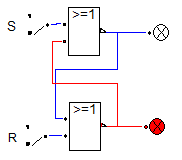
\includegraphics[width=0.3\columnwidth]{DT3Graphics/SR-FF-NOR.PNG}
\captionof{figure}{Realisierung in NOR-Technik}
\vspace{20mm}
Charakteristische Gleichung des SR-Flip-Flops als disjunktive Normalform:
\begin{equation}
	Q\textsubscript{n+1}:=( S\wedge \overline{R})\vee (\overline{R} \wedge Q \textsubscript{n})
\end{equation}
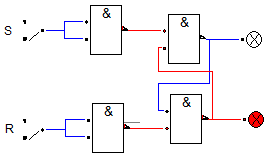
\includegraphics[width=0.4\columnwidth]{DT3Graphics/SR-FF-NAND.PNG}
\captionof{figure}{Realisierung in NAND-Technik}
\end{center}
\subsection*{Arbeitsweise}
Liegt an beiden Eingängen (S und R) eine null an tritt der Speicherfall ein, das heißt der Zustand bleibt. Liegt an S eine null und an R eine eins an, schaltet der Flip-Flop unabhängig von dem vorherigen Zustand auf null (Rücksetzen). Liegt an S eine eins und an R eine null an, schaltet der Flip-Flop auf eins (Setzen). Dass an beiden Eingängen eine eins anliegt ist der verbotene Fall. 
\begin{center}
\section{E-Flip-Flop}
\begin{tabular}{c|c|c|c|c}
E1&E2&Q\textsubscript{n}&Q\textsubscript{n+1}&Bemerkung\\
\hline
0&0&0&0&Speichern\\
0&0&1&1&Speichern\\
0&1&0&0&Rücksetzen\\
0&1&1&0&Rücksetzen\\
1&0&0&1&Setzen\\
1&0&1&1&Setzen\\
1&1&0&0&Speichern\\
1&1&1&1&Speichern\\
\end{tabular}
\captionof{table}{Wahrheitstabelle E-Flip-Flop}
\vspace{20mm}
\begin{tabular}{c|c|c|c|c}
\diagbox{Q\textsubscript{n}}{E1E2}&00&01&11&10\\
\hline
0& & & &1\\
\hline
1&1&&1&1\\
\end{tabular}
\captionof{table}{KV-Diagramm E-Flip-Flop}
\vspace{20mm}
Charakteristische Gleichung des E-Flip-Flops als konjunktive Normalform:
\begin{equation}
	Q\textsubscript{n+1}:=( \overline{E1} \vee E2)\wedge (\overline{E1}\vee \overline{Q \textsubscript{n}}) \wedge (E2 \vee \overline{Q \textsubscript{n}})
\end{equation}
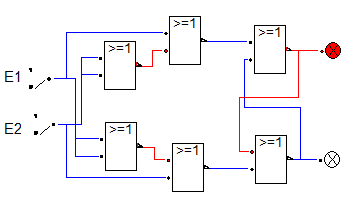
\includegraphics[width=0.5\columnwidth]{DT3Graphics/E-FF-NOR.PNG}
\captionof{figure}{Realisierung in NOR-Technik}
\vspace{20mm}
Charakteristische Gleichung des E-Flip-Flops als disjunktive Normalform:
\begin{equation}
	Q\textsubscript{n+1}:=( E1\wedge \overline{E2})\vee (E1 \wedge Q \textsubscript{n}) \vee (\overline{E2} \wedge Q \textsubscript{n})
\end{equation}
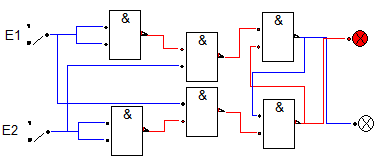
\includegraphics[width=0.5\columnwidth]{DT3Graphics/E-FF-NAND.PNG}
\captionof{figure}{Realisierung in NAND-Technik}
\vspace{-5mm}
\end{center}
\subsection*{Arbeitsweise}
Der E-Flip-Flop ist ein erweiteter SR-Flip-Flop. Der einzige Unterschied ist, dass es den verbotenen Fall nicht gibt. Liegt an beiden Eingängen eine eins an, speichert der E-Flip-Flop.
\begin{center}
\section{D-Flip-Flop}
\begin{tabular}{c|c|c|c|c}
D&C&Q\textsubscript{n}&Q\textsubscript{n+1}&Bemerkung\\
\hline
0&0&0&0&Speichern\\
0&0&1&1&Speichern\\
0&1&0&0&Rücksetzen\\
0&1&1&0&Rücksetzen\\
1&0&0&0&Speichern\\
1&0&1&1&Speichern\\
1&1&0&1&Setzen\\
1&1&1&1&Setzen\\
\end{tabular}
\captionof{table}{Wahrheitstabelle D-Flip-Flop}

\vspace{15mm}

\begin{tabular}{c|c|c|c|c}
\diagbox{Q\textsubscript{n}}{DC}&00&01&11&10\\
\hline
0& & &1& \\
\hline
1&1& &1&1\\
\end{tabular}
\captionof{table}{KV-Diagramm D-Flip-Flop}

\vspace{15mm}

Charakteristische Gleichung des D-Flip-Flops als konjunktive Normalform:
\begin{equation}
	Q\textsubscript{n+1}:=( \overline{D} \vee \overline{Q \textsubscript{n}})\wedge (\overline{D}\vee \overline{C}) \wedge (C \vee \overline{Q \textsubscript{n}})
\end{equation}

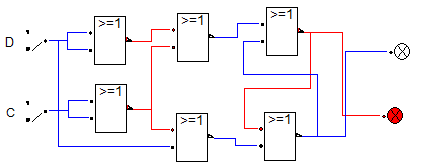
\includegraphics[width=0.5\columnwidth]{DT3Graphics/D-FF-NOR.PNG}
\captionof{figure}{Realisierung in NOR-Technik}
\vspace{20mm}
Charakteristische Gleichung des D-Flip-Flops als disjunktive Normalform:
\begin{equation}
	Q\textsubscript{n+1}:=( D\wedge Q \textsubscript{n} )\vee (D \wedge C) \vee (\overline{C} \wedge Q \textsubscript{n})
\end{equation}
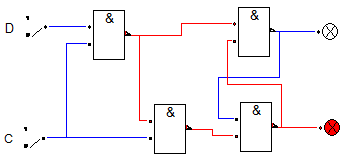
\includegraphics[width=0.5\columnwidth]{DT3Graphics/D-FF-NAND.PNG}
\captionof{figure}{Realisierung in NAND-Technik}
\vspace{10mm}
\end{center}
\subsection*{Arbeitsweise}
Der D-Flip-Flop ist ein taktzustandsgesteuerter Flip-Flop. Das heißt, dass am Takt eine eins anliegen muss, damit der Flip-Flop setzt oder rücksetzt. Liegt am Takt Eingang C eine null an wird gespeichert. Liegt an C eine eins und an D eine null an, tritt der Rücksetzen Fall ein. Es wird also auf null geschaltet. Liegt an C und D eine eins an, wird der Flip-Flop gesetzt, also schaltet er auf eins.
\begin{center}
\newpage
\section{T-Flip-Flop}
\begin{tabular}{c|c|c|c}
T&Q\textsubscript{n}&Q\textsubscript{n+1}&Bemerkung\\
\hline
0&0&0&Speichern\\
0&1&1&Speichern\\
1&0&1&Umschalten\\
1&1&0&Umschalten\\

\end{tabular}
\captionof{table}{Wahrheitstabelle T-Flip-Flop}
\vspace{10mm}
\begin{tabular}{c|c|c}
\diagbox{Q\textsubscript{n}}{T}&0&1\\
\hline
0& &1\\
\hline
1&1& \\
\end{tabular}
\captionof{table}{KV-Diagramm T-Flip-Flop}
\vspace{10mm}

Charakteristische Gleichung des T-Flip-Flops als konjunktive Normalform:
\begin{equation}
	Q\textsubscript{n+1}:=( T \vee \overline{Q \textsubscript{n}})\wedge (\overline{T} \vee  Q \textsubscript{n})
\end{equation}
\vspace{5mm}

Charakteristische Gleichung des T-Flip-Flops als disjunktive Normalform:
\begin{equation}
	Q\textsubscript{n+1}:=( \overline{T}\wedge Q \textsubscript{n} )\vee (T \wedge \overline{Q \textsubscript{n}}) 
\end{equation}

\section{JK-Flip-Flop}
\begin{tabular}{c|c|c|c|c}
J&K&Q\textsubscript{n}&Q \textsubscript{n+1}&Bemerkung\\
\hline
0&0&0&0&save\\
0&0&1&1&save\\
0&1&0&0&kill\\
0&1&1&0&kill\\
1&0&0&1&jump\\
1&0&1&1&jump\\
1&1&0&0&toggle\\
1&1&1&1&toggle\\
\end{tabular}
\captionof{table}{Wahrheitstabelle JK-Flip-Flop}
\begin{tabular}{c|c|c|c}
J&K&Q \textsubscript{n+1}&Bemerkung\\
\hline
0&0&Q\textsubscript{n}&save\\
0&1&0&kill\\
1&0&1&jump\\
1&1&$\overline{\hbox{Q \textsubscript{n}}}$&toggle\\
\end{tabular}
\captionof{table}{Komprimierte Wahrheitstabelle JK-Flip-Flop}
\vspace{10mm}
\begin{tabular}{c|c|c|c|c}
\diagbox{Q\textsubscript{n}}{JK}&00&01&11&10\\
\hline
0& & &1&1\\
\hline
1&1& & &1\\
\end{tabular}
\captionof{table}{KV-Diagramm JK-Flip-Flop}
\vspace{10mm}
Charakteristische Gleichung des JK-Flip-Flops als konjunktive Normalform:
\begin{equation}
	Q\textsubscript{n+1}:=( \overline{J} \vee Q \textsubscript{n})\wedge (\overline{J}\vee K) \wedge (K \vee \overline{Q \textsubscript{n}})
\end{equation}
\vspace{5mm}

Charakteristische Gleichung des JK-Flip-Flops als disjunktive Normalform:
\begin{equation}
	Q\textsubscript{n+1}:=( J\wedge \overline{Q \textsubscript{n}} )\vee (J \wedge \overline{K}) \vee (\overline{K} \wedge Q \textsubscript{n})
\end{equation}
\end{center}
\newpage
\chapter{Kritische Schlussbetrachtung}
\section{Olbrich, Marie}
 In Versuch DT3 wurden verschiedene Flip-Flop-Arten (SR-Flip-Flop, E-Flip-Flop, D-Flip-Flop) untersucht. Dabei sollten Unterschiede zwischen den Flip-Flops festgestellt werden. \par
In der Vorbereitung wurden dazu zunächst Wahrheitstabellen und KV-Diagramme der Flip-Flops ausgefüllt um die konjunktive und disjunktive Normalform zu bilden. Um die disjunktive Normalform zu erhalten, wurden die Einsen im KV-Diagramm zusammenfasst. Um auf die konjunktive Normalform zu kommen, wurde die disjunktive Normalform negiert. Eine Alternative um die konjunktive Normalform zu bilden ist, die Nullen im KV-Diagramm zusammenzufassen. Mit Hilfe der beiden Normalformen wurden Schaltungen in NOR- und NAND-Technik entwickelt. \par
Bei der Versuchsdurchführung wurden mit Hilfe eines HPS-Boards, wie in Abbildung 2.1 zu sehen, ICs und Laborleitungen die verschiedenen Schaltungen aufgebaut und auf ihre Funktion getestet. Dabei musste die Pin Belegung der ICs beachtet werden. \par
Alle in der Versuchsanleitung beschriebenen Aufgaben konnten ohne größere Probleme in der gegebenen Zeit durchgeführt werden.\\
\vspace{10mm}
\begin{center}
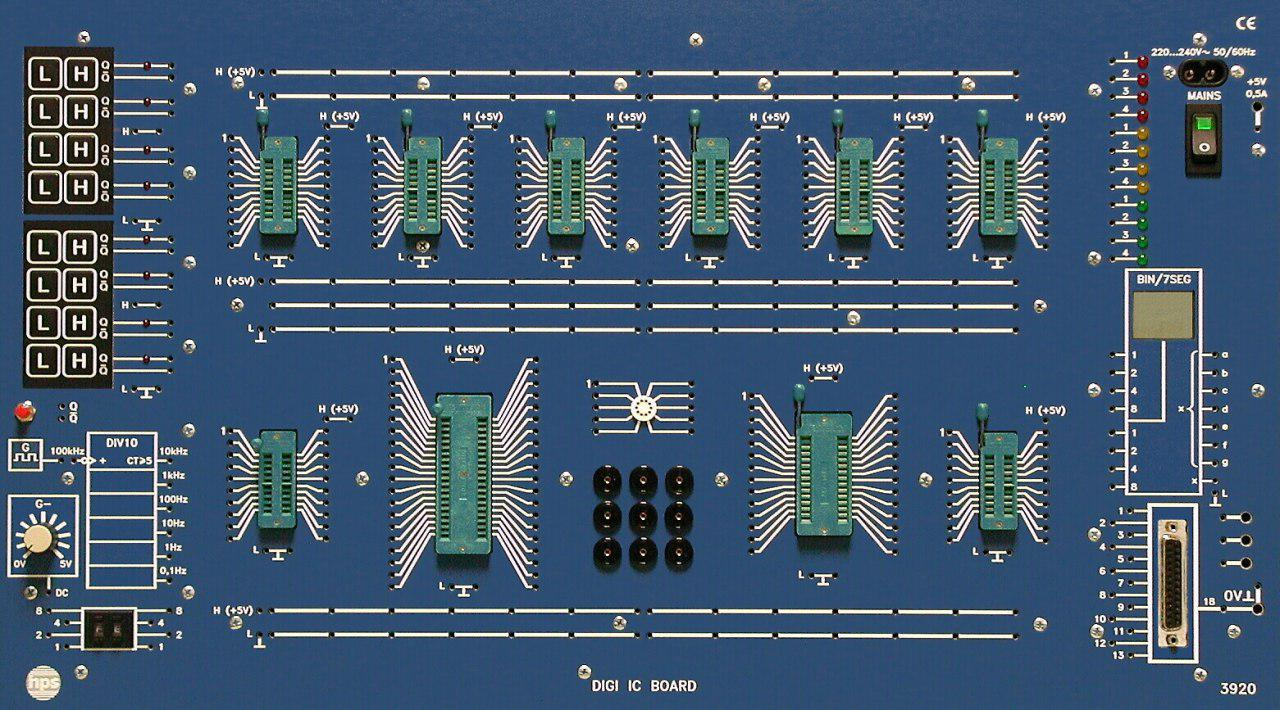
\includegraphics[width=0.75\columnwidth]{DT3Graphics/HPSBoard.jpg}
\captionof{figure}{HPS-Board}
\end{center}

\section{Hoffmann, Manuel}
 Die zugrunde liegenden vorbereitenden Aufgaben beginnen damit, dass zu erst die Wahrheitstabellen
der einzelnen Flip-Flop typen erarbeitet werden. \par
Im zweiten Schritt sind die KV-Diagramme und daraus resultierend die konjunktive sowie die disjunktive 
Normalform der Schaltgleichung der FF´s zu erstellen.
Die disjunktive Normalform wird gebildet indem man die ``1'' Einträge aus den KV-Diagrammen zusammenfast.
Die konjunktive Normalform bildet man indem man die ``0'' Einträge der KV-Diagramme zusammenfast, 
alternativ ist es möglich die disjunktive Normalform, unter beauchtung der Schaltalgebraischen regeln, zu negieren.\par
Abschließend sind, aus den KV-Diagrammen und aus der konjunktiven sowie disjunktiven Normalform, schaltungen mit NOR- 
und NAND-Bausteinen zu den einzelnen Flip-Flops zu erstellen.\par
Bei dem Laborversuch selbst werden, unter zuhilfenahme eines HPS-Boards sowie IC´s und Laborleitungen, die Schaltungen nachgebaut und einer Abnahme in form eines Funktionstest unterzogen.\par
Alle gestellten Aufgaben wurden in der gegebenen Zeit erfolgreich bearbeitet.
Das einzige Problem das auftrat ergab sich durch eine Fehlinterpretation der Aufgabenstellung zu der theoretischen 
erstellung der Schaltungen. 
Es wurden nicht wie vorgesehen Schaltungen mit einem Ausgang ``Q'' erstellt sondern wie 
Technisch und in der gägingen Literatur üblich mit zwei Ausgängen ``Q'' und ``nicht-Q''.
\chapter{Literaturverzeichnis}
Klaus Beuth: Digitaltechnik, Vogel, 13. Auflage, 2006



%%%%%%%%%%%%%%%%%%%%%%%%%%%%%%%%%%%%%%%%%%%%%%%%%%%%%%%%%%%%%%%%%%%%%%%%%%%%%%%%%%%%%%%
%%%%%%%%%%%%%%%%%%%%%%%%%%%%%%%%%%%%%%%%%%%%%%%%%%%%%%%%%%%%%%%%%%%%%%%%%%%%%%%%%%%%%%%
%%%%%%%%%%%%%%%%%%%%%%%%%%%%%%%%%%%%%%%%%%%%%%%%%%%%%%%%%%%%%%%%%%%%%%%%%%%%%%%%%%%%%%%
%%%%%%%%%%%%%%%%%%%%%%%%%%%%% Hier fängt der Text an %%%%%%%%%%%%%%%%%%%%%%%%%%%%%%%%%%
%%%%%%%%%%%%%%%%%%%%%%%%%%%%%%%%%%%%%%%%%%%%%%%%%%%%%%%%%%%%%%%%%%%%%%%%%%%%%%%%%%%%%%%
%%%%%%%%%%%%%%%%%%%%%%%%%%%%%%%%%%%%%%%%%%%%%%%%%%%%%%%%%%%%%%%%%%%%%%%%%%%%%%%%%%%%%%%
%%%%%%%%%%%%%%%%%%%%%%%%%%%%%%%%%%%%%%%%%%%%%%%%%%%%%%%%%%%%%%%%%%%%%%%%%%%%%%%%%%%%%%%

\end{document}